\documentclass[10pt]{article}
\usepackage{longtable}
\usepackage{float}
\usepackage{wrapfig}
\usepackage{rotating}
\usepackage[normalem]{ulem}
\usepackage{amsmath}
\usepackage{textcomp}
\usepackage{marvosym}
\usepackage{wasysym}
\usepackage{amssymb}
\usepackage{hyperref}
\usepackage{color,soul} % for highlighting
\usepackage{graphicx}
\graphicspath{{/Users/benjaminbass/seacloud/class/earthMaterials/picBank/}}

\usepackage{frame,color}
\usepackage{framed}
\usepackage{minibox}

% \usepackage[T1]{fontenc}
% \usepackage{tilting} %bring title up
% \setlength{\droptitle}{-10cm}

\usepackage[version=3]{mhchem}
% How to Use MChem
% \ce{SO4^2-}
% \ce{^{227}_{90}Th+}
% \ce{A\bond{-}B\bond{=}C\bond{#}D}
% \ce{CO2 + C -> 2CO}
% \ce{SO4^2- + Ba^2+ -> BaSO4 v}


\author{Benjamin Bass}
\date{2 March 2016}
\title{\vspace{-2.0cm}Biotite} %bring title up temporary Fix

\begin{document}

\maketitle

% \framebox{Use frameboxes until figure out alignmen}

\begin{center}
  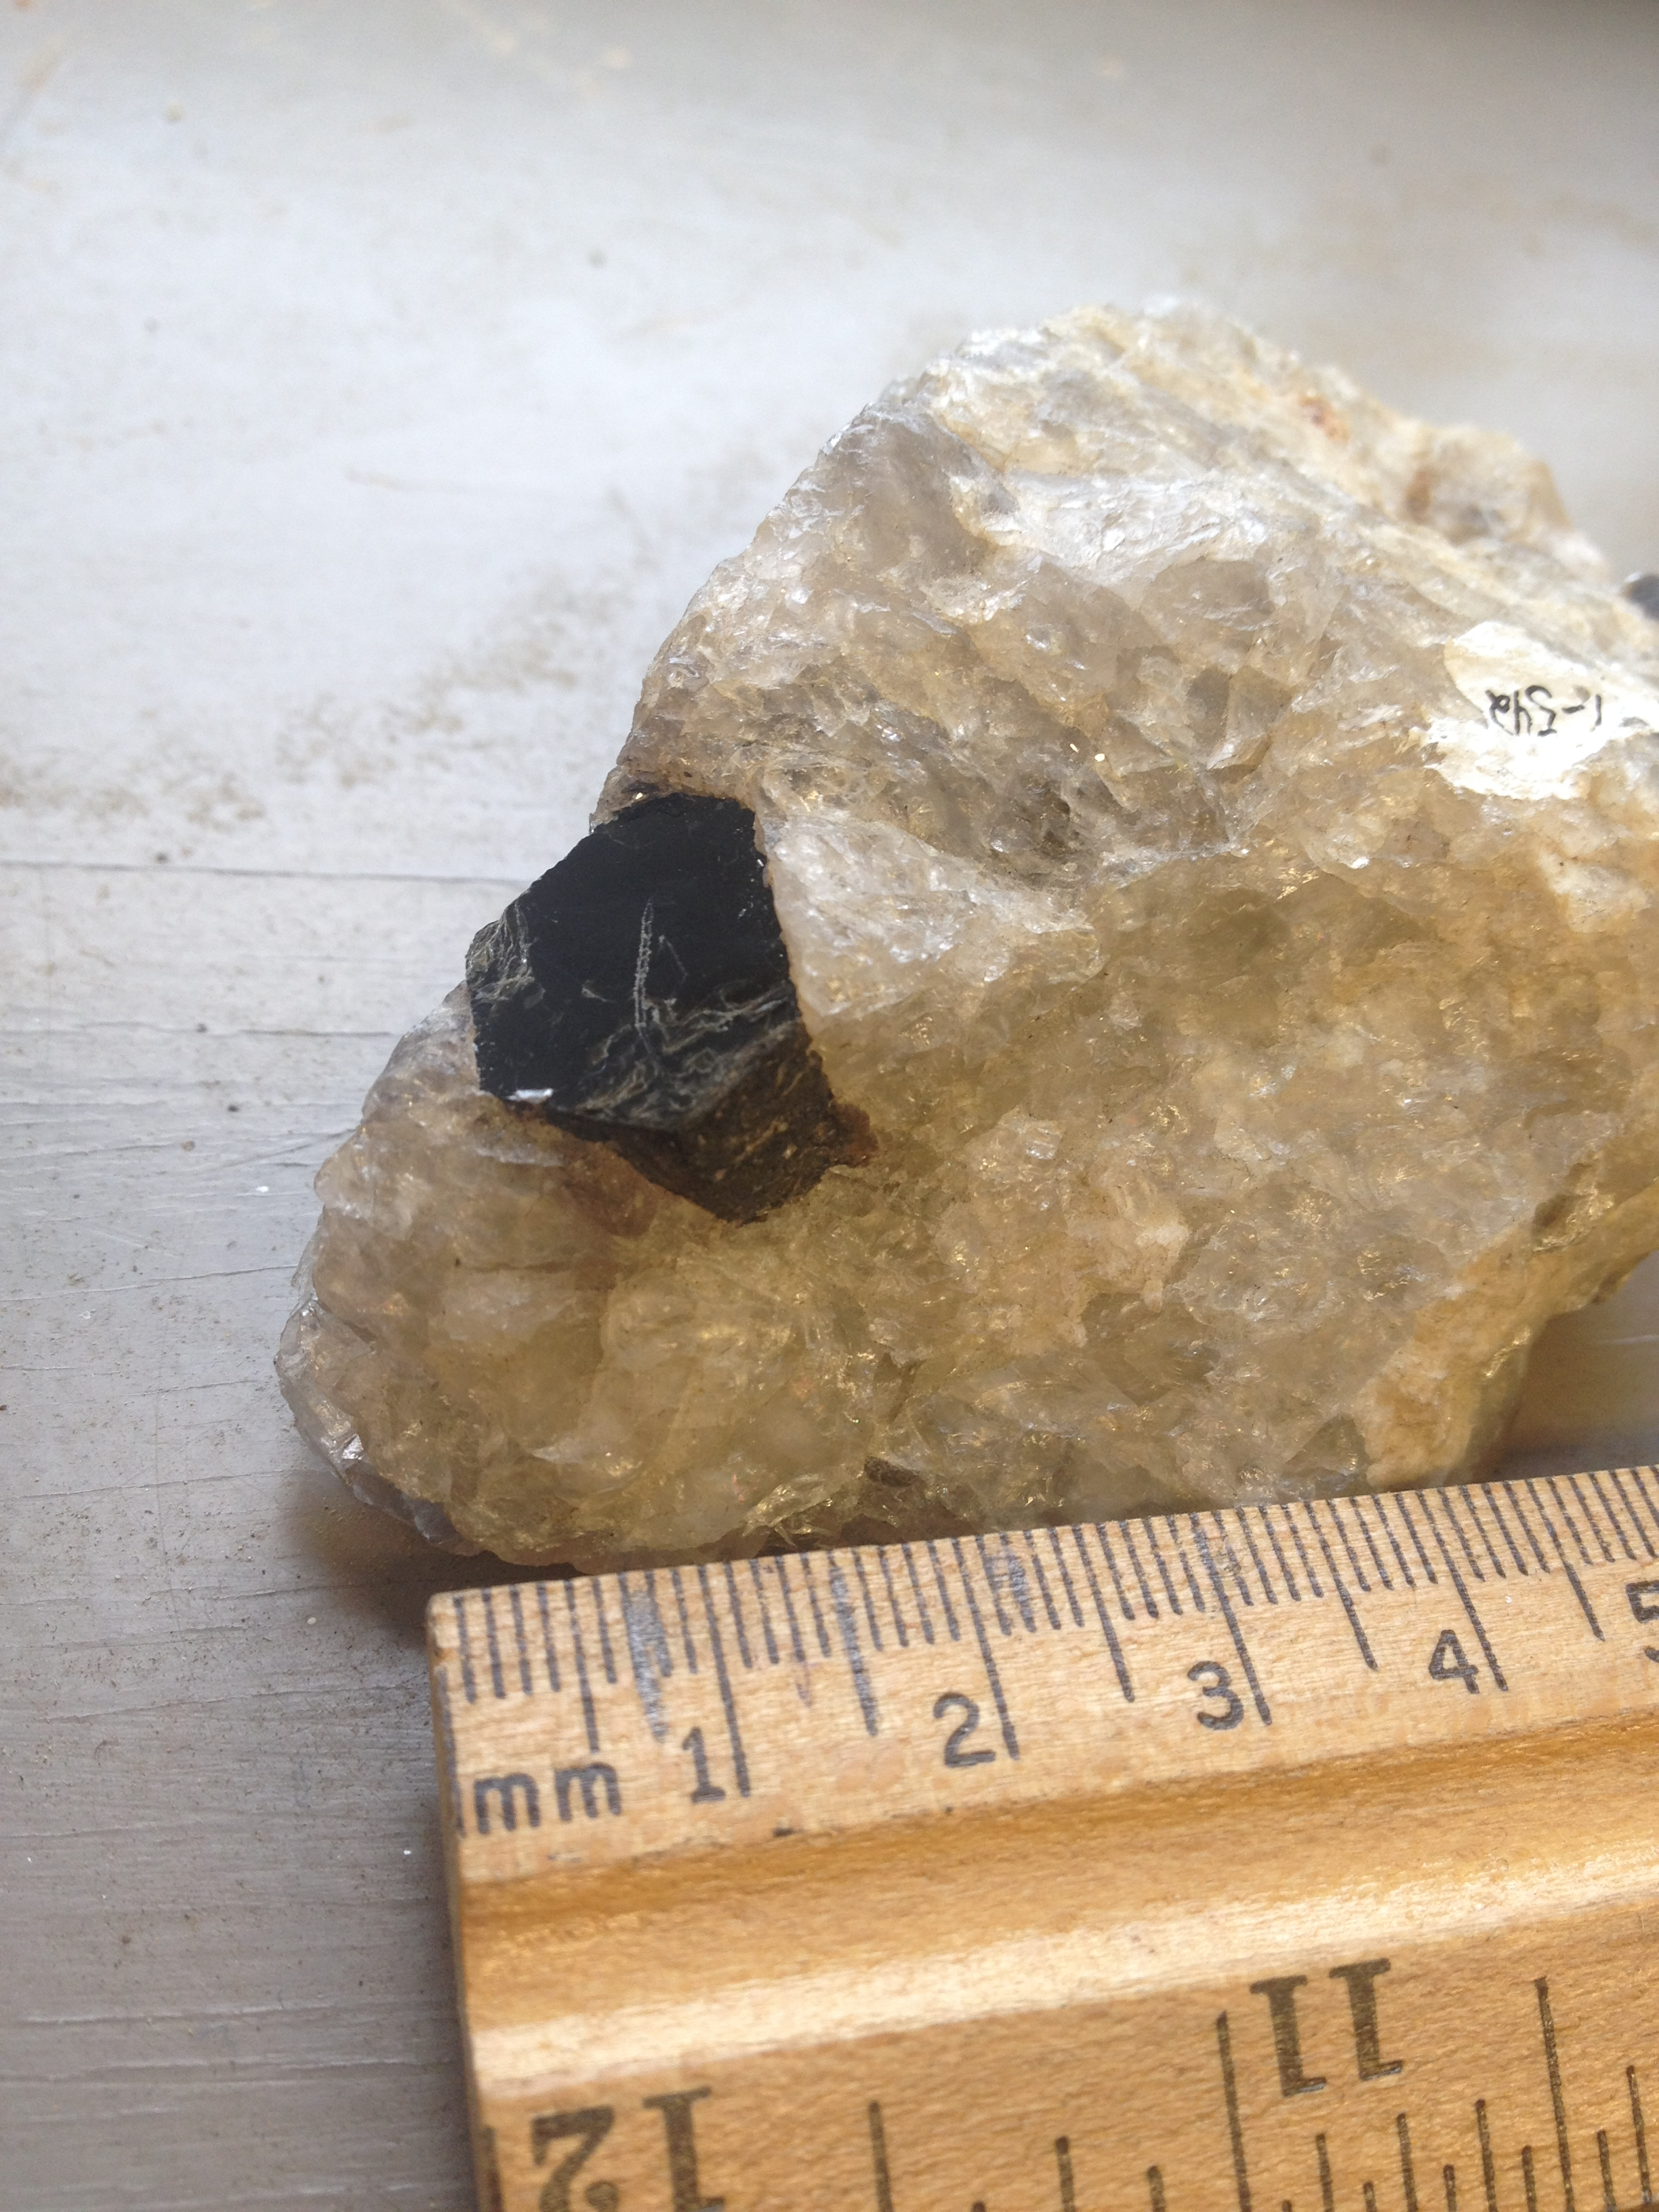
\includegraphics[scale=.05]{biotite1}\footnote{Cleavage produces thin elastic folia.}
  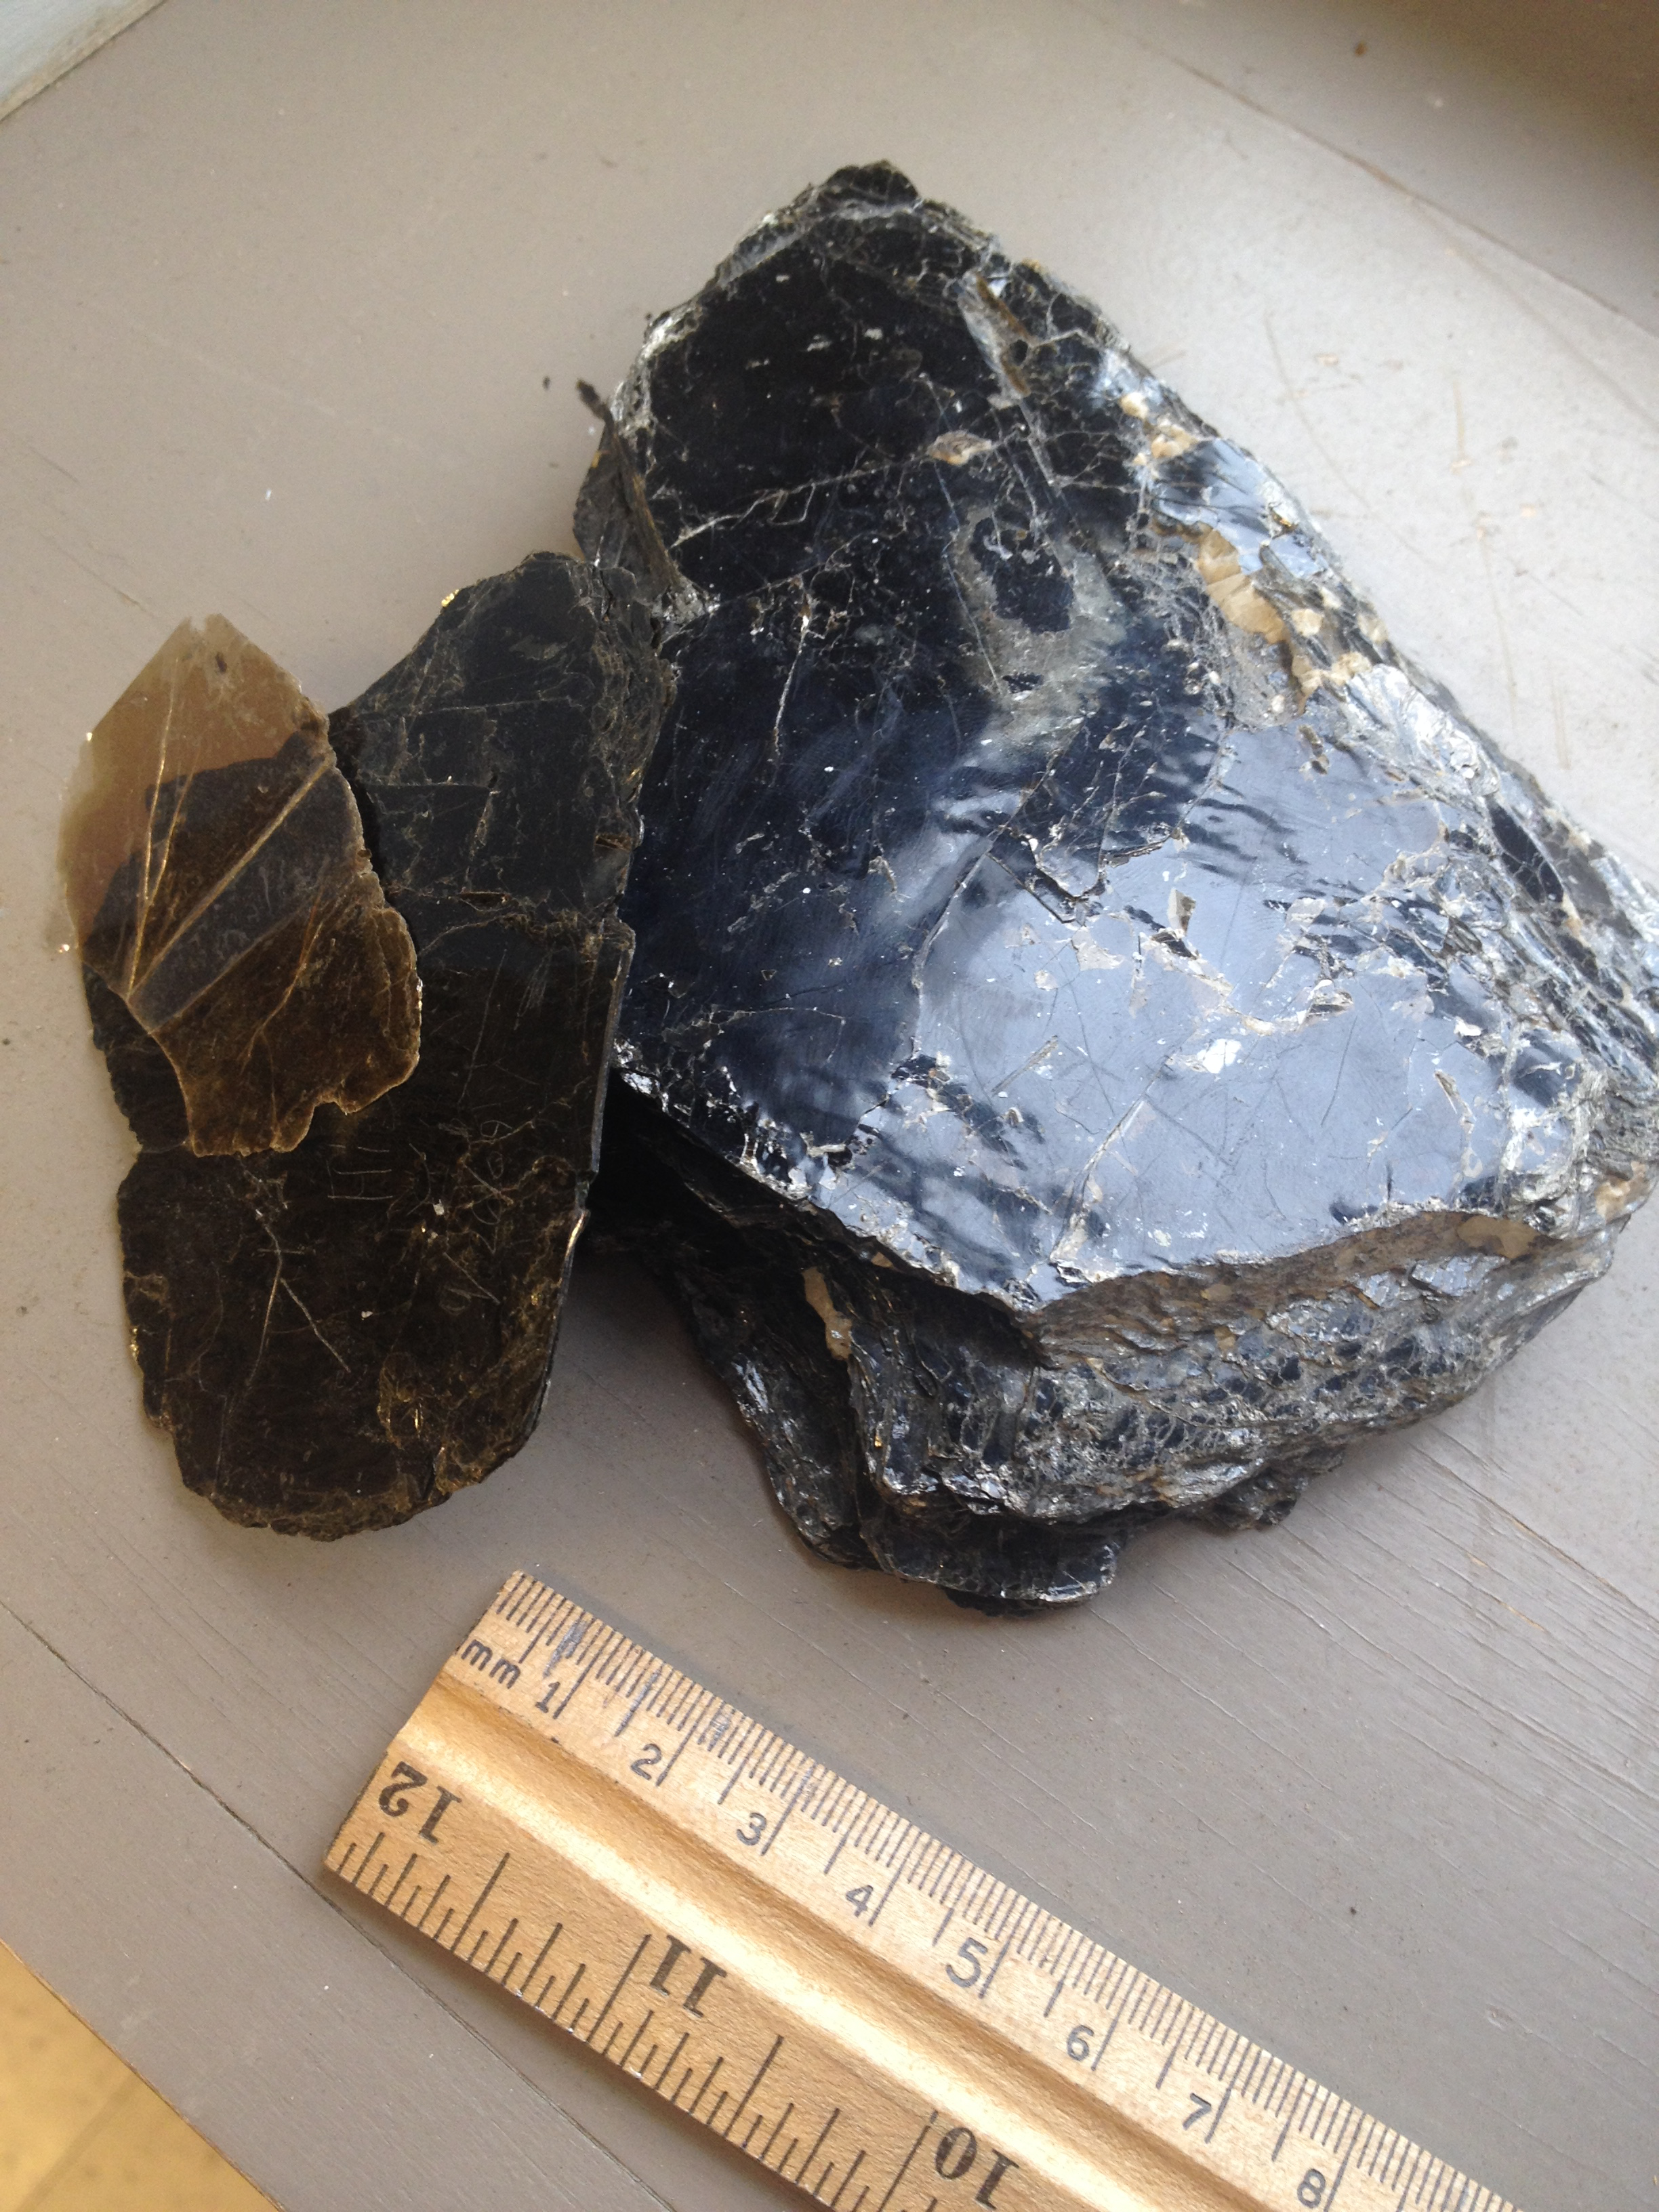
\includegraphics[scale=.05]{biotite2}\footnote{Black and vitreous in hand sample}
\end{center}



\framebox[15cm][l]{\textbf{General Mineral Formula}: $K(Fe,Mg)_{3}AlSi_{3}O_{10}(OH)_{2}$ }\
\framebox[15cm][l]{\textbf{Mineral Chemical Class}: Phyllosilicates }\
\framebox[15cm][l]{\textbf{Specific Gravity}: 2.9 - 3.2 }\
\framebox[15cm][l]{\textbf{Hardness}: 5-6 }\
\framebox[15cm][l]{\textbf{Cleavage}: \hl{2,2 prismatic} }\
\framebox[15cm][l]{\textbf{Luster}: Vitreous, silky }\
\framebox[15cm][l]{\textbf{Streak}: Colorless }\
\framebox[15cm][l]{\textbf{Characteristic Color(s)}: \hl{White, light to dark grey. \& many in between.} }\
\framebox[15cm][l]{\textbf{Crystal System}: Monoclinic }\
\framebox[15cm][l]{\textbf{Crystal Class}: 2/\it{m} }\

\begin{framed}
  \textbf{Crystal Description (common forms, habit, etc.)}: \hl{As elongated prismatic crystals. in bladed groups. Columnous, fibrous. Also radiating as wheat sheaf formations in thin, hairlike masses and tough interlocking fibers.}
\end{framed}

\begin{framed}
  \textbf{Environment (where you find the material}: In contact menamorphic rocks in hronfels and skarns. Serpentine deposits. Commonly marble of metamorphasized calcite.
\end{framed}

\begin{framed}
  \textbf{Common Mineral Associations (in samples, also consult text, notes}: Albite, Barite, Chlorite, Epidote, Muscovite.
\end{framed}

\begin{framed}
  \textbf{Scientific Usage/Significance}: Prone to dramatic expansion when heated.
\end{framed}

\begin{framed}
  \textbf{Industrial or Social Use/Significance}: Additive in pot soil for expansion.
\end{framed}

\begin{framed}
  \textbf{Environmental Significance}: Weathered Vermiculite can expand and is an important part of soils.
\end{framed}

% Possible other Solutions
% \framebox(300,20){\minibox{\textbf{R-Sq}:For example}}

\end{document}
%%% Local Variables:
%%% mode: latex
%%% TeX-master: t
%%% End:
